% ============================================================================
% LC3 CC531 A Analisis en Macrodatos 2026-2 — Informe
% Dataset: Denuncias por desaparicion de personas [MININTER] 2019-2024
% Compilar:  latexmk -pdf informe.tex     (o pdflatex 3 veces)
% ============================================================================
\documentclass[10pt,a4paper]{article}
\usepackage[spanish,english]{babel}
\usepackage[utf8]{inputenc}
\usepackage[T1]{fontenc}
\usepackage{indentfirst}
\usepackage{anysize}
\marginsize{2.5cm}{1.8cm}{1.5cm}{1.7cm}
\usepackage{amssymb}
\usepackage{amsfonts}
\usepackage{amsmath}
\usepackage{amsthm}
\usepackage{multicol}
\usepackage{multirow}
\usepackage{graphicx}
\usepackage[hidelinks]{hyperref}
\usepackage[htt]{hyphenat}
\usepackage{caption}
\usepackage{subcaption}
\usepackage{tocloft}
\usepackage{longtable}
\usepackage{booktabs}
\usepackage{array}
\usepackage{listings}
\usepackage{xcolor}
\usepackage{float}
\usepackage{tikz}
\usepackage{pgfplots}
\pgfplotsset{compat=1.18}

\renewcommand{\cftsecleader}{\cftdotfill{\cftdotsep}}
\theoremstyle{definition}
\renewcommand{\thefootnote}{\fnsymbol{footnote}}

\lstdefinestyle{scala}{
  language=Java,
  basicstyle=\ttfamily\scriptsize,
  keywordstyle=\color{blue!70!black},
  commentstyle=\color{green!40!black}\itshape,
  stringstyle=\color{red!60!black},
  numbers=left, numberstyle=\tiny\color{gray},
  breaklines=true, frame=single, rulecolor=\color{gray!50},
  backgroundcolor=\color{gray!5},
  showstringspaces=false, tabsize=2
}
\lstdefinestyle{sql}{
  language=SQL,
  basicstyle=\ttfamily\scriptsize,
  keywordstyle=\color{blue!70!black}\bfseries,
  commentstyle=\color{green!40!black}\itshape,
  numbers=left, numberstyle=\tiny\color{gray},
  breaklines=true, frame=single, rulecolor=\color{gray!50},
  backgroundcolor=\color{gray!5},
  showstringspaces=false
}

\title{Detecci\'on de patrones en las denuncias por desaparici\'on de personas en el Per\'u (2019--2024) con Spark y PostgreSQL}
\date{Noviembre 2026}
\hypersetup{pdftitle={LC3 CC531 - Denuncias por desaparicion de personas},pdfauthor={Arbues Perez, Sergio Sebastian Pezo Jimenez}}

\begin{document}
\sloppy

\maketitle

\begin{center}
  Estudiantes:\\
  \vspace{5pt}
  {\large Arbu\'es Enrique P\'erez Villanueva \quad Sergio Sebastian Pezo Jimenez}\\
  Universidad Nacional de Ingenier\'ia, Facultad de Ciencias,\\
  e-mails: arbues.perez.v@uni.pe \quad sergio.pezo.j@uni.pe
\end{center}
\vspace{5pt}
\begin{center}
  Curso:\\
  \vspace{5pt}
  {\large CC531 A -- An\'alisis en Macrodatos (2026-2)}\\
  {\large Laboratorio 03}
\end{center}
\vspace{20pt}

\begin{abstract}
{\small
\hspace*{0.5cm}
Se analizan 93,831 registros de denuncias por desaparici\'on de personas publicados por el
Ministerio del Interior en la Plataforma Nacional de Datos Abiertos, correspondientes a las
121,427 personas reportadas como desaparecidas entre enero de 2019 y diciembre de 2024. El
trabajo cubre las tres capas exigidas: (i) cinco consultas implementadas con la API de RDD de
Spark y el paradigma mapReduce, (ii) un modelo estrella cargado en PostgreSQL 16 mediante un
proceso ETL documentado, y (iii) veinte consultas con la API de DataFrame de Spark SQL, seis de
ellas con vistas temporales y \texttt{spark.sql}, cuyos resultados se exportan a Excel usando
Spark. Cada consulta declara su objetivo, la pregunta de negocio que responde, la soluci\'on
implementada, las columnas empleadas y la interpretaci\'on del resultado.

\textbf{Palabras clave:} Spark, RDD, mapReduce, Spark SQL, PostgreSQL, datos abiertos, seguridad ciudadana.
}
\end{abstract}

\pagenumbering{arabic}
\tableofcontents

\vspace{20pt}
\hrule
\vspace{10pt}

% ============================================================================
\section{Introducci\'on}
% ============================================================================
La desaparici\'on de personas es uno de los delitos que m\'as afecta la confianza en las
instituciones: cada denuncia implica una familia que busca a alguien y un aparato estatal que
debe priorizar la b\'usqueda. El Ministerio del Interior (MININTER) publica el registro de estas
denuncias en la Plataforma Nacional de Datos Abiertos (PNDA), con detalle de fecha, ubigeo del
hecho y perfil de la persona (sexo, rango de edad, estado civil, nacionalidad, nivel educativo y
ocupaci\'on).

El objetivo del laboratorio es recorrer el ciclo completo de un proyecto de macrodatos sobre ese
registro: describir la fuente, almacenarla en una base relacional con un modelo definido por el
grupo, y responder 25 preguntas distintas con tres tecnolog\'ias de c\'omputo distribuidas ---
RDD con mapReduce, la API de DataFrame y SQL sobre vistas temporales --- verificando en cada caso
que el resultado sea interpretable.

\section{Marco te\'orico}

\subsection{El fen\'omeno y su teor\'ia de datos}
El dataset describe \emph{hechos} de desaparici\'on, no personas individuales. Cada fila es una
combinaci\'on \'unica de \emph{dimensi\'on temporal} (a\~no y mes), \emph{dimensi\'on
geogr\'afica} (ubigeo, departamento, provincia, distrito) y \emph{dimensiones del perfil de la
v\'ictima} (sexo, rango de edad, estado civil, nacionalidad, nivel educativo, ocupaci\'on), con
una \emph{medida} aditiva: la cantidad de personas denunciadas en ese cruce. La teor\'ia
subyacente es la de un modelo multidimensional (Kimball): un hecho central y dimensiones que lo
describen, con la cantidad como medida y las jerarqu\'ias geogr\'afica y etaria como ejes de
an\'alisis. Esta estructura es la que permite responder tanto preguntas de agregaci\'on simple
(cu\'antas personas por departamento) como de composici\'on (qu\'e porcentaje son menores) y de
cobertura (qu\'e territorios o meses no tienen registros).

\subsection{RDD, mapReduce y DataFrame}
Un RDD (\emph{Resilient Distributed Dataset}) es una colecci\'on inmutable y particionada de
objetos, tolerante a fallos por linaje. El paradigma \emph{mapReduce} se implementa con
\texttt{map} (transformar cada elemento en un par clave-valor) y \texttt{reduceByKey} (agregar
por clave), lo que obliga a un \emph{shuffle} para reunir las claves. La API de DataFrame, en
cambio, describe la consulta como un \'arbol l\'ogico que el optimizador Catalyst reescribe y
convierte en c\'odigo (Tungsten), con lo que se obtiene el mismo resultado con menos c\'odigo y
mejor plan f\'isico. Las vistas temporales permiten registar un DataFrame en el cat\'alogo de la
sesi\'on y consultarlo con SQL est\'andar.

% ============================================================================
% Seccion 2 — Descripcion del dataset (punto 2 del enunciado)
% ============================================================================
\section{Descripci\'on del dataset}

\subsection{Ficha t\'ecnica}

\begin{center}
\begin{tabular}{p{4.2cm}p{10.5cm}}
\toprule
\textbf{Nombre} & Denuncias por desaparici\'on de personas \\
\textbf{Organizaci\'on} & Ministerio del Interior del Per\'u (MININTER) \\
\textbf{Rubro PNDA} & Seguridad y Justicia \\
\textbf{Fuente} & Plataforma Nacional de Datos Abiertos
  (\url{https://www.datosabiertos.gob.pe/dataset/denuncias-por-desaparici\%C3\%B3n-de-personas-mininter}) \\
\textbf{Recurso analizado} & \texttt{BD\_DESAPARICIONES\_ENERO\_2019\_DICIEMBRE\_2024.csv} (8.1 MB) \\
\textbf{Actualizaci\'on del recurso} & 18 de setiembre de 2026 \\
\textbf{Cobertura} & enero 2019 -- diciembre 2024 (72 meses) \\
\textbf{Grano} & a\~no $\times$ mes $\times$ ubigeo del hecho $\times$ perfil de la v\'ictima \\
\textbf{Registros} & 93,831 filas \\
\textbf{Columnas} & 13 \\
\textbf{Medida} & \texttt{CANTIDAD}: personas denunciadas en ese cruce (1 a 18; total 121,427) \\
\textbf{Formato} & CSV separado por comas, codificaci\'on UTF-8 con BOM, fin de l\'inea CRLF \\
\textbf{Recursos complementarios} & diccionario de datos (\texttt{.xlsx}) y metadatos (\texttt{.docx}) \\
\bottomrule
\end{tabular}
\end{center}

\subsection{Teor\'ia que implican los datos}
El registro no contiene personas identificables: contiene \emph{hechos de desaparici\'on
agregados}. Cada fila es el cruce de una fecha (a\~no y mes), una ubicaci\'on del hecho (ubigeo,
departamento, provincia, distrito) y un perfil de la v\'ictima (sexo, rango de edad, estado
civil, nacionalidad, nivel educativo y ocupaci\'on), con la cantidad de personas denunciadas en
ese cruce como medida. Es, por tanto, un cubo de datos en forma plana: el hecho es la
desaparici\'on, las dimensiones describen el cu\'ando, el d\'onde y el qui\'en, y la medida es
aditiva, lo que permite totalizar por cualquiera de las dimensiones sin recalcular el dataset.

Desde la pol\'itica p\'ublica, los datos responden a la teor\'ia de la \emph{b\'usqueda urgente}:
la probabilidad de encontrar a una persona desaparecida cae r\'apidamente con las horas, por lo
que el inter\'es anal\'itico se concentra en la distribuci\'on territorial (d\'onde se denuncia
m\'as), en el perfil etario (las y los adolescentes son el grupo m\'as expuesto) y en la
estacionalidad (meses con m\'as carga operativa para las comisar\'ias).

\subsection{Campos, cardinalidad y valores vac\'ios}

\begin{center}
\small
\begin{tabular}{llrp{6.6cm}}
\toprule
\textbf{Campo} & \textbf{Tipo} & \textbf{Valores} & \textbf{Descripci\'on y observaciones}\\
\midrule
A\~NO & entero & 6 & 2019 a 2024. Distribuci\'on de registros: 18,934 / 14,373 / 15,728 / 14,916 / 14,607 / 15,273.\\
MES & entero & 12 & 1 a 12. Los 72 cruces a\~no-mes tienen registros.\\
UBIGEO\_HECHO & texto & 1,506 & C\'odigo de 6 d\'igitos (departamento-provincia-distrito), con ceros a la izquierda que se conservan como texto. Un mismo ubigeo (150121) aparece con dos nombres de distrito: PUEBLO LIBRE y MAGDALENA VIEJA (su nombre antiguo).\\
DPTO\_HECHO & texto & 26 & Incluye ``LIMA METROPOLITANA'' y ``REGI\'ON LIMA'' como unidades separadas, y ``CALLAO'' como departamento.\\
PROV\_HECHO & texto & 195 & Nombre de la provincia del hecho.\\
DIST\_HECHO & texto & 1,506 & Nombre del distrito del hecho.\\
SEXO & texto & 3 & F (54,595), M (39,162) y 74 vac\'ios (0.08\,\%).\\
RANGO\_EDAD & texto & 7 & 0-5, 6-11, 12-17 (45,303 registros, el 48.3\,\%), 18-29, 30-59, 60 a m\'as y 1,243 vac\'ios (1.3\,\%).\\
EST\_CIVIL & texto & 7 & Soltero(a) 63,583; NO INDICA 8,286; casado(a) 6,147; conviviente, divorciado(a), viudo(a); 13,480 vac\'ios (14.4\,\%).\\
NACIONALIDAD & texto & 57 & Per\'u 91,171 (97.2\,\%), Venezuela 2,118, Colombia 123, Ecuador 70, Chile 54.\\
NIVEL\_EDUCATIVO & texto & 6 & Secundaria 21,782, primaria 9,195, superior 1,157, t\'ecnica, sin instrucci\'on; 60,731 vac\'ios (64.7\,\%).\\
OCUPACION & texto & 289 & Estudiante 20,894 (22.3\,\%), ama de casa 2,808, independiente 1,272; 60,790 vac\'ios (64.8\,\%).\\
CANTIDAD & entero & 18 & Personas denunciadas en el registro: 1 (78,128 registros, 83.3\,\%), 2, 3, \dots hasta 18 como m\'aximo.\\
\bottomrule
\end{tabular}
\end{center}

\subsection{Reglas de los datos identificadas}
\begin{enumerate}
  \item \textbf{La medida es positiva y acotada.} \texttt{CANTIDAD} toma valores entre 1 y 18; no
        hay ceros ni negativos, por lo que la suma de la columna es directamente el total de
        personas (121,427).
  \item \textbf{Un registro no equivale a una persona.} El 83.3\,\% de las filas tiene
        \texttt{CANTIDAD} = 1; contar filas (93,831) subestimar\'ia el fen\'omeno en 27,596
        personas. Toda consulta del informe agrega con \texttt{SUM(CANTIDAD)}.
  \item \textbf{El ubigeo es un identificador textual y tiene una excepci\'on.} Tiene ceros a la
        izquierda (por ejemplo \texttt{021809} para Nuevo Chimbote, \'Ancash); leerlo como
        n\'umero lo corromper\'ia. El ubigeo \texttt{150121} aparece con dos nombres de distrito
        (PUEBLO LIBRE y su antiguo nombre, MAGDALENA VIEJA), lo que obliga a colapsar la
        dimensi\'on geogr\'afica a una fila por ubigeo antes de hacer joins.
  \item \textbf{Las ausencias son informativas, no aleatorias.} Nivel educativo y ocupaci\'on
        faltan en cerca del 65\,\% de los registros, y faltan juntos (mismo patr\'on de 60,731 y
        60,790 vac\'ios), lo que sugiere un formulario que solo se completa en algunas
        comisar\'ias. No se imput\'o: se etiquet\'o como \texttt{NO ESPECIFICA}.
  \item \textbf{Nacionalidad no es sin\'onimo de migrante.} ``PER\'U'' es un valor m\'as de la
        columna; para analizar poblaci\'on extranjera hay que excluirlo expl\'citamente.
  \item \textbf{El territorio es jer\'arquico.} Los 1,506 ubigeos se agrupan en 195 provincias y
        26 unidades departamentales, lo que permite clasificarlas por regi\'on natural (costa,
        sierra, selva) sin informaci\'on externa.
  \item \textbf{No hay duplicados exactos de la llave completa.} Las 93,831 filas son
        combinaciones distintas de fecha, ubigeo y perfil.
\end{enumerate}

\subsection{Identidad del dataset y no duplicidad}
El registro se publica en la PNDA como un \emph{dataset independiente}: tiene su propia URL,
su propio identificador en el portal, su diccionario de datos (\texttt{.xlsx}) y su documento de
metadatos (\texttt{.docx}), y no figura como subconjunto declarado de otro dataset del cat\'alogo.
Su sistema de origen es el SIDPOL del MININTER, que alimenta tambi\'en otros registros policiales
publicados por separado (denuncias policiales, indicadores de seguridad ciudadana); lo que se
analiza aqu\'i es el registro de desapariciones publicado como tal, con su propia cobertura
(enero 2019 -- diciembre 2024) y sus 13 campos.

Se deja constancia de dos decisiones para que el trabajo sea trazable:
\begin{itemize}
  \item Se usa \textbf{un solo recurso} (el de 13 columnas, 2019--2024). El portal publica
        adem\'as un recurso 2019--2025 de 10 columnas que, en los seis a\~nos comparables, suma
        exactamente lo mismo por a\~no (0.00 de diferencia). Apilar ambos duplicar\'ia todos los
        casos, de modo que se eligi\'o el recurso con mayor detalle de columnas.
  \item No se imputan valores ni se excluyen filas por tener campos vac\'ios; esas ausencias se
        documentan como regla del dato (secci\'on 2.4) y se conservan como categor\'ia
        \texttt{NO ESPECIFICA}.
\end{itemize}

\subsection{Informaci\'on que se puede obtener}
Con este registro se pueden responder, entre otras, las siguientes l\'ineas de an\'alisis, que
son las que estructuran las 25 consultas del laboratorio:
\begin{itemize}
  \item \textbf{Concentraci\'on territorial}: qu\'e distritos, provincias y departamentos acumulan
        m\'as personas desaparecidas y cu\'al es su peso relativo.
  \item \textbf{Perfil de la v\'ictima}: distribuci\'on por sexo, grupo etario, estado civil,
        nivel educativo y ocupaci\'on, y combinaciones entre ellos.
  \item \textbf{Vulnerabilidad de menores}: proporci\'on de menores de 18 a\~nos por departamento
        y comparaci\'on con la poblaci\'on adulta.
  \item \textbf{Tendencia y estacionalidad}: evoluci\'on anual, variaci\'on interanual mes a mes e
        \'indice de cada mes frente al esperado.
  \item \textbf{Migraci\'on}: peso y evoluci\'on de las personas de nacionalidad extranjera.
  \item \textbf{Calidad y cobertura}: meses o territorios sin registros, integridad referencial
        del cat\'alogo geogr\'afico y efecto del periodo pand\'emico (2020--2021).
\end{itemize}


% ============================================================================
% Seccion 4 — Proceso ETL para la base de datos (punto 4 del enunciado)
% ============================================================================
\section{Proceso ETL para la base de datos}

\subsection{Arquitectura de tablas definida por el grupo}
Se eligi\'o un \textbf{modelo estrella} porque el dataset ya viene en forma de cubo: la tabla de
hechos guarda la medida (\texttt{cantidad}) y las claves de las dimensiones, y cada dimensi\'on
guarda los atributos con los que se agrupa o filtra. Las claves primarias son naturales
(el propio valor del dataset), lo que hace el ETL verificable: cualquier fila del CSV se puede
seguir hasta la tabla de hechos.

\begin{figure}[H]
\centering
\begin{tikzpicture}[
  every node/.style={font=\scriptsize},
  dim/.style={draw, fill=blue!6, rounded corners=2pt, inner sep=3pt, align=left, text width=3.5cm},
  fac/.style={draw, fill=orange!12, rounded corners=2pt, inner sep=4pt, align=left, text width=4.4cm},
  link/.style={-latex, gray!70!black}
]
\node[fac] (hecho) at (0,0) {
  \textbf{hecho\_desaparicion}\\
  \rule{4.2cm}{0.2pt}\\
  id (PK)\\
  anio (FK), mes\\
  ubigeo (FK)\\
  sexo (FK)\\
  rango\_edad (FK)\\
  estado\_civil (FK)\\
  nacionalidad (FK)\\
  nivel\_educativo (FK)\\
  ocupacion (FK)\\
  \textbf{cantidad}
};
\node[dim] (tiempo) at (-5.6, 2.6) {\textbf{dim\_tiempo}\\ anio (PK)\\ periodo\\ es\_pandemia};
\node[dim] (geo)    at (5.6, 2.6)  {\textbf{dim\_geografia}\\ ubigeo (PK)\\ departamento\\ provincia\\ distrito\\ region\_natural\\ cod\_departamento\\ cod\_provincia};
\node[dim] (edad)   at (-5.6, -0.6) {\textbf{dim\_rango\_edad}\\ rango\_edad (PK)\\ grupo\_etario\\ orden\\ edad\_min, edad\_max};
\node[dim] (sexo)   at (-5.6, -3.0) {\textbf{dim\_sexo}\\ sexo (PK)\\ descripcion};
\node[dim] (civil)  at (5.6, -0.7) {\textbf{dim\_estado\_civil}\\ estado\_civil (PK)};
\node[dim] (nacion) at (5.6, -3.0) {\textbf{dim\_nacionalidad}\\ nacionalidad (PK)\\ es\_extranjera};
\node[dim] (nivel)  at (-5.6, -5.2) {\textbf{dim\_nivel\_educativo}\\ nivel\_educativo (PK)\\ orden};
\node[dim] (ocup)   at (5.6, -5.2) {\textbf{dim\_ocupacion}\\ ocupacion (PK)};
\draw[link] (tiempo) -- (hecho);
\draw[link] (geo) -- (hecho);
\draw[link] (edad) -- (hecho);
\draw[link] (sexo) -- (hecho);
\draw[link] (civil) -- (hecho);
\draw[link] (nacion) -- (hecho);
\draw[link] (nivel) -- (hecho);
\draw[link] (ocup) -- (hecho);
\end{tikzpicture}
\caption{Diagrama entidad-relaci\'on del modelo estrella implementado en PostgreSQL 16.
\texttt{hecho\_desaparicion} referencia las ocho dimensiones; \texttt{dim\_geografia} tiene una
fila por ubigeo (1,506).}
\label{fig:er}
\end{figure}

Adem\'as del modelo final se cre\'o una tabla de \textbf{staging} (\texttt{stg\_desaparicion})
con las 13 columnas tal como llegan del CSV. Esta tabla materializa el paso de extracci\'on y
permite reejecutar la transformaci\'on sin volver a descargar el archivo.

\subsection{Extracci\'on}
El dataset se descarga del portal de la PNDA como un \'unico CSV de 8.1 MB. La extracci\'on se
hace con \texttt{COPY} de PostgreSQL, que es la v\'ia m\'as r\'apida para archivos locales y no
requiere herramientas externas:

\begin{lstlisting}[style=sql]
COPY stg_desaparicion (anio, mes, ubigeo_hecho, dpto_hecho, prov_hecho, dist_hecho,
                       sexo, rango_edad, est_civil, nacionalidad, nivel_educativo,
                       ocupacion, cantidad)
FROM '/home/arbues/macrodatos/PC3/data/denuncias_desaparicion_2019_2024.csv'
WITH (FORMAT csv, HEADER true, DELIMITER ',', ENCODING 'UTF8', NULL '');
\end{lstlisting}

\subsection{Transformaci\'on}
Sobre la tabla de staging se aplican seis reglas, todas verificables en \texttt{sql/02\_etl.sql}:

\begin{enumerate}
  \item \textbf{Categ\'oricas vac\'ias a \texttt{NO ESPECIFICA}}: se aplica a \texttt{sexo},
        \texttt{rango\_edad}, \texttt{est\_civil}, \texttt{nacionalidad},
        \texttt{nivel\_educativo} y \texttt{ocupacion}. No se imputa ning\'un valor del dataset.
  \item \textbf{Ubigeo}: se normaliza a 6 caracteres con \texttt{LPAD} y se agrupa por ubigeo
        tomando un solo nombre por distrito, porque el c\'odigo \texttt{150121} aparece con dos
        graf\'ias (PUEBLO LIBRE y MAGDALENA VIEJA). Sin este paso, cada join con la dimensi\'on
        geogr\'afica duplicar\'ia 82 personas.
  \item \textbf{Regi\'on natural}: se deriva del departamento con una regla \texttt{CASE}
        (12 departamentos de costa, 10 de sierra, 4 de selva).
  \item \textbf{Periodo pand\'emico}: 2019 = pre-pandemia, 2020--2021 = pandemia,
        2022--2024 = post-pandemia.
  \item \textbf{Grupo etario}: los seis rangos del dataset se agrupan en primera infancia, ni\~nez,
        adolescente, adulto joven, adulto y adulto mayor, con un orden num\'erico para ordenar
        resultados sin depender del texto.
  \item \textbf{Filtro de calidad}: solo se cargan hechos con \texttt{cantidad} positiva y no
        nula (en la pr\'actica, el 100\,\% de las filas).
\end{enumerate}

\subsection{Llenado}
El orden de carga respeta las dependencias: primero las ocho dimensiones y despu\'es la tabla de
hechos, todo dentro de una sola transacci\'on para que el ETL sea at\'omico. Las dimensiones se
pueblan con \texttt{INSERT \dots SELECT DISTINCT} sobre el staging, de modo que el cat\'alogo
geogr\'afico (1,506 ubigeos) y los cat\'alogos de nacionalidad (57 valores) y ocupaci\'on (289
valores) se generan del propio dataset.

\begin{lstlisting}[style=sql]
BEGIN;
TRUNCATE stg_desaparicion;
COPY stg_desaparicion (...) FROM :'ruta_csv' WITH (FORMAT csv, HEADER true, ...);
INSERT INTO dim_tiempo ...;
INSERT INTO dim_geografia (...) SELECT DISTINCT ... FROM stg_desaparicion WHERE ubigeo <> '';
INSERT INTO dim_rango_edad ...; INSERT INTO dim_sexo ...;
INSERT INTO dim_nacionalidad (...) SELECT DISTINCT ... ON CONFLICT DO NOTHING;
INSERT INTO dim_ocupacion (...)    SELECT DISTINCT ... ON CONFLICT DO NOTHING;
INSERT INTO hecho_desaparicion (...)
SELECT ... FROM stg_desaparicion WHERE cantidad > 0;
COMMIT;
\end{lstlisting}

\subsection{Verificaci\'on del ETL}
El script cierra con tres controles que se muestran en las capturas de la base de datos
funcionando (\texttt{evidencias/pg-*.png}):
\begin{itemize}
  \item conteo de filas por tabla: \texttt{hecho\_desaparicion} = 93,831,
        \texttt{dim\_geografia} = 1,506, \texttt{dim\_nacionalidad} = 57,
        \texttt{dim\_ocupacion} = 289;
  \item control de cuadre: \texttt{SUM(cantidad)} = 121,427, id\'entico al calculado en Spark;
  \item consulta de comprobaci\'on sobre la vista \texttt{v\_desaparicion} (top 10 de
        departamentos por personas), que devuelve exactamente el mismo orden que la consulta
        5a.1 ejecutada en Spark.
\end{itemize}

\IfFileExists{../evidencias/pg-version.png}{
\begin{figure}[H]
\centering
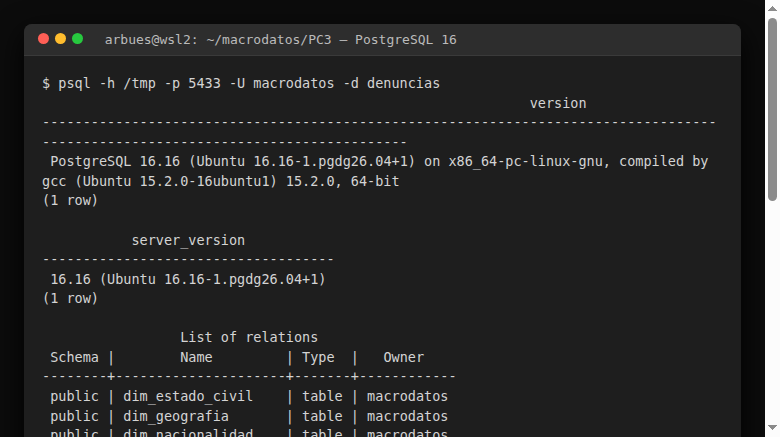
\includegraphics[width=0.9\textwidth]{../evidencias/pg-version.png}
\caption{Servidor PostgreSQL 16 en funcionamiento y verificaci\'on de la versi\'on.}
\end{figure}}{}

\IfFileExists{../evidencias/pg-conteos.png}{
\begin{figure}[H]
\centering
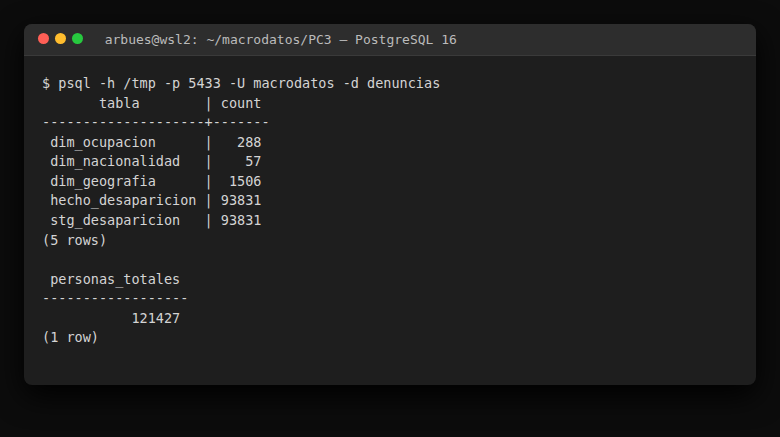
\includegraphics[width=0.9\textwidth]{../evidencias/pg-conteos.png}
\caption{Conteos por tabla y control de cuadre del ETL (121,427 personas).}
\end{figure}}{}

\IfFileExists{../evidencias/pg-consulta.png}{
\begin{figure}[H]
\centering
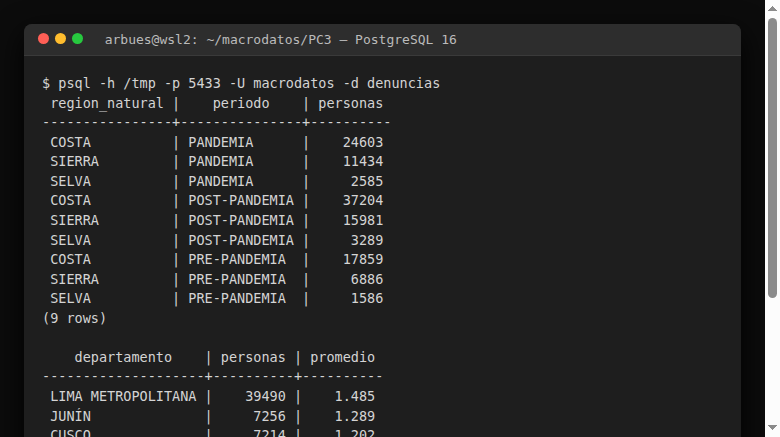
\includegraphics[width=0.9\textwidth]{../evidencias/pg-consulta.png}
\caption{Consulta de comprobaci\'on sobre la vista \texttt{v\_desaparicion}.}
\end{figure}}{}


\section{Metodolog\'ia}

\subsection{Entorno y versiones}
El trabajo se ejecut\'o en una m\'aquina con WSL2 (Ubuntu) usando exactamente las versiones de
clase: Spark 3.3.2 con Scala 2.12.15 y OpenJDK 11, PostgreSQL 16 y el driver JDBC
\texttt{postgresql-42.7.6}. Las 25 consultas se ejecutan con \texttt{spark-shell} en modo
\texttt{local[*]}, es decir, con paralelismo sobre los n\'ucleos de la m\'aquina.

\subsection{Organizaci\'on del c\'odigo}
\begin{center}
\begin{tabular}{ll}
\toprule
Ruta & Contenido\\
\midrule
\texttt{code/comun/esquema.scala} & lectura, limpieza, dimensiones y vistas temporales\\
\texttt{code/rdd/*.scala} & consultas 3a, 3b y 3c (mapReduce)\\
\texttt{code/sql/*.scala} & consultas 5a--5g (DataFrame, vistas y Excel)\\
\texttt{sql/01\_ddl.sql} & arquitectura de tablas en PostgreSQL\\
\texttt{sql/02\_etl.sql} & proceso ETL completo (staging $\to$ dimensiones $\to$ hechos)\\
\texttt{excel/*.xlsx} & resultados de 5e y 5f exportados con Spark\\
\texttt{evidencias/salidas/*.txt} & salida real de cada consulta\\
\texttt{bin/ejecutar.sh} & ejecutor: \texttt{:load esquema.scala} + consulta\\
\bottomrule
\end{tabular}
\end{center}

\subsection{Tratamiento de datos vac\'ios}
Cinco campos categ\'oricos llegan vac\'ios en una parte de los registros: \texttt{NIVEL\_EDUCATIVO}
(64.7\,\%), \texttt{OCUPACION} (64.8\,\%), \texttt{EST\_CIVIL} (14.4\,\%), \texttt{RANGO\_EDAD}
(1.3\,\%) y \texttt{SEXO} (0.08\,\%). No se imput\'o ning\'un valor: se cre\'o la categor\'ia
expl\'icita \texttt{NO ESPECIFICA}, que se conserva en todos los agregados y se declara en cada
interpretaci\'on para no sesgar los porcentajes. Un solo registro no tiene \texttt{UBIGEO\_HECHO};
se mantiene en la tabla de hechos con geograf\'ia nula, lo que se refleja en el LEFT JOIN de la
consulta 5c.2.

% ============================================================================
% Seccion 4 — Las 25 consultas (parte 1: RDD y DataFrame 5a-5c)
% ============================================================================
\section{Resultados y discusi\'on: las 25 consultas}

En esta secci\'on se documenta cada consulta con la estructura que exige el punto 7 del
enunciado: tipo de pregunta, la pregunta en lenguaje natural, la soluci\'on implementada, las
columnas y filas involucradas, las partes importantes del c\'odigo y la interpretaci\'on del
resultado. Todas las cifras provienen de la ejecuci\'on real registrada en
\texttt{evidencias/salidas/}.

\subsection{Consultas con mapReduce (punto 3)}

\subsubsection*{3-a \textbar{} M\'aximo y m\'inimo de personas por sexo}
\begin{description}
\item[Tipo de pregunta] agregaci\'on con extremos (max/min) por categor\'ia, en RDD.
\item[Pregunta] \emph{Para cada sexo, cu\'al es el mayor y el menor n\'umero de personas
      desaparecidas registrado en un solo hecho, y d\'onde ocurri\'o?}
\item[Soluci\'on] tres jobs de \texttt{mapReduce}: (1) \texttt{map} a pares
      \texttt{(sexo, (cantidad, cantidad))} y \texttt{reduceByKey} que se queda con el m\'aximo y
      el m\'inimo; (2) y (3) \texttt{map} a \texttt{(sexo, tupla del registro)} y
      \texttt{reduceByKey} que conserva el registro con la cantidad mayor (y menor).
\item[Columnas usadas] \texttt{SEXO} (clave), \texttt{CANTIDAD} (medida), y
      \texttt{DPTO\_HECHO}, \texttt{PROV\_HECHO}, \texttt{DIST\_HECHO}, \texttt{A\~NO},
      \texttt{MES} para ubicar el registro extremo.
\item[C\'odigo clave]
\begin{lstlisting}[style=scala]
hechos.map(h => (h.sexo, (h.cantidad, h.cantidad)))
      .reduceByKey((a, b) => (math.max(a._1, b._1), math.min(a._2, b._2)))
\end{lstlisting}
\item[Resultado]
\begin{center}
\begin{tabular}{lp{5.6cm}rr}
\toprule
Sexo & Registro del m\'aximo & M\'ax. & M\'in.\\
\midrule
F & LIMA METROPOLITANA / LIMA / VILLA MAR\'IA DEL TRIUNFO (2019-11) & 18 & 1\\
M & CUSCO / CUSCO / SANTIAGO (2019-10) & 14 & 1\\
NO ESPECIFICA & LIMA METROPOLITANA / LIMA / SAN MART\'IN DE PORRES (2019-12) & 3 & 1\\
\bottomrule
\end{tabular}
\end{center}
\item[Interpretaci\'on] El registro extremo de todo el dataset son \textbf{18 personas
      desaparecidas en un solo hecho}, en Villa Mar\'ia del Triunfo en noviembre de 2019, y
      corresponde a mujeres. Los m\'inimos valen 1 en los tres casos, lo que confirma que la
      unidad m\'inima de registro es la persona. El patr\'on de fondo es que el 83.3\,\% de los
      93,831 registros tiene una sola persona, as\'i que la distribuci\'on es muy asim\'etrica:
      los hechos con 5 o m\'as personas son solo 1,400 registros, pero aportan 9,188 personas.
\end{description}

\subsubsection*{3-b \textbar{} Promedio, mediana, desviaci\'on, mayor y menor de la cantidad}
\begin{description}
\item[Tipo de pregunta] estad\'istica descriptiva de una variable num\'erica, en RDD.
\item[Pregunta] \emph{Cu\'antas personas desaparecen en promedio en un hecho registrado, cu\'al
      es el valor t\'ipico y cu\'anto se dispersa la serie?}
\item[Soluci\'on] cuatro jobs: (1) un solo \texttt{reduce} que acumula \texttt{(suma, conteo)}
      para el promedio; (2) un \texttt{reduce} de la suma de cuadrados para la desviaci\'on
      ($\sigma^2 = E[x^2] - \bar{x}^2$); (3) ordenamiento con \texttt{sortBy} + \texttt{zipWithIndex}
      y \texttt{filter} de las dos posiciones centrales para la mediana; (4) \texttt{reduce} con
      \texttt{math.max} y \texttt{math.min}. Se adopta la lectura de ``media'' como
      \emph{mediana}, tal como se declara en el marco metodol\'ogico.
\item[Columnas usadas] \texttt{CANTIDAD} \'unicamente (93,831 filas).
\item[C\'odigo clave]
\begin{lstlisting}[style=scala]
val sumaConteo = hechos.map(h => (h.cantidad.toDouble, 1L))
                       .reduce((a, b) => (a._1 + b._1, a._2 + b._2))
val sumaCuadrados = hechos.map(h => h.cantidad.toDouble * h.cantidad.toDouble).reduce(_ + _)
val medios = hechos.map(_.cantidad.toDouble).sortBy(x => x).zipWithIndex()
                   .filter(p => p._2 == n / 2 || p._2 == (n - 1) / 2).map(_._1).collect()
\end{lstlisting}
\item[Resultado]
\begin{center}
\begin{tabular}{lr@{\hspace{2cm}}lr}
\toprule
Registros ($n$) & 93,831 & Promedio & 1.2941\\
Suma de personas & 121,427 & Mediana & 1.00\\
Mayor & 18 & Desviaci\'on poblacional & 0.8906\\
Menor & 1 & Varianza poblacional & 0.7931\\
\bottomrule
\end{tabular}
\end{center}
\item[Interpretaci\'on] El valor t\'ipico es \textbf{una persona por hecho} (mediana = 1) y el
      promedio es 1.29: la diferencia entre ambos confirma la asimetr\'ia hacia la derecha. La
      desviaci\'on de 0.89 es casi tan grande como el promedio, se\~nal de alta heterogeneidad
      (existen hechos con 18 personas). Desagregado por sexo, los registros de mujeres tienen
      promedio 1.3715 y desviaci\'on 1.0454, mientras que los de hombres tienen 1.1866 y 0.5971:
      los hechos m\'ultiples son mucho m\'as frecuentes entre v\'ictimas mujeres, lo que es
      consistente con desapariciones de grupos familiares o de adolescentes.
\end{description}

\subsubsection*{3-c.1 \textbar{} Porcentaje de menores de 18 a\~nos por departamento}
\begin{description}
\item[Tipo de pregunta] participaci\'on porcentual (decimales) con tres mapReduce encadenados.
\item[Pregunta] \emph{Qu\'e porcentaje de las desapariciones de cada departamento corresponde a
      menores de 18 a\~nos y qu\'e departamentos concentran el mayor peso relativo de poblaci\'on
      infantil y adolescente?}
\item[Soluci\'on] MR1 calcula el total por departamento; MR2 calcula el total de menores
      (rangos 0-5, 6-11 y 12-17) por departamento; MR3 hace el \texttt{join} de ambos RDD y
      calcula el porcentaje, que es la salida decimal.
\item[Columnas usadas] \texttt{DPTO\_HECHO} (clave), \texttt{RANGO\_EDAD} (filtro),
      \texttt{CANTIDAD} (medida).
\item[C\'odigo clave]
\begin{lstlisting}[style=scala]
val mr1Total   = hechos.map(h => (h.departamento, h.cantidad)).reduceByKey(_ + _)
val mr2Menores = hechos.filter(h => Lc3.MENORES.contains(h.rangoEdad))
                       .map(h => (h.departamento, h.cantidad)).reduceByKey(_ + _)
val mr3 = mr1Total.join(mr2Menores)
                  .map { case (d, (t, m)) => (d, t, m, dosDec(m * 100.0 / t)) }
\end{lstlisting}
\item[Resultado] Total nacional: 70,178 menores de 18 sobre 121,427 personas =
      \textbf{57.79\,\%}. Extremos: MADRE DE DIOS 72.21\,\% (473 de 655), UCAYALI 70.74\,\%,
      LORETO 70.25\,\%, TUMBES 69.03\,\%, CAJAMARCA 68.97\,\%; en el otro extremo LIMA
      METROPOLITANA 50.02\,\%, AREQUIPA 52.27\,\%, PUNO 52.60\,\%, TACNA 54.10\,\%.
\item[Interpretaci\'on] M\'as de la mitad de las personas desaparecidas son menores de edad, y
      la condici\'on no se reparte de forma homog\'enea: en la selva y en la sierra rural
      (Madre de Dios, Ucayali, Loreto, Cajamarca) casi 7 de cada 10 desapariciones son de
      menores, mientras que en Lima Metropolitana la proporci\'on baja a la mitad. Es el
      hallazgo con mayor implicancia de pol\'itica p\'ublica del an\'alisis: la b\'usqueda
      urgente de menores deber\'ia priorizarse en las regiones amaz\'onicas, no donde hay m\'as
      casos absolutos.
\end{description}

\subsubsection*{3-c.2 \textbar{} Porcentaje de personas extranjeras por a\~no}
\begin{description}
\item[Tipo de pregunta] participaci\'on porcentual anual y variaci\'on interanual, con tres
      mapReduce.
\item[Pregunta] \emph{Qu\'e porcentaje de las denuncias corresponde a personas de nacionalidad
      extranjera cada a\~no y c\'omo var\'ia ese porcentaje?}
\item[Soluci\'on] MR1 total por a\~no; MR2 total de extranjeros (nacionalidad distinta de
      \texttt{PER\'U}) por a\~no; MR3 \texttt{join} de los dos agregados para obtener el
      porcentaje y su diferencia en puntos porcentuales respecto del a\~no anterior.
\item[Columnas usadas] \texttt{A\~NO} (clave), \texttt{NACIONALIDAD} (filtro),
      \texttt{CANTIDAD} (medida).
\item[Resultado]
\begin{center}
\begin{tabular}{rrrrr}
\toprule
A\~no & Total & Extranjeros & \% & Variaci\'on (pp)\\
\midrule
2019 & 26,331 & 434 & 1.65 & --\\
2020 & 18,481 & 316 & 1.71 & +0.06\\
2021 & 20,141 & 397 & 1.97 & +0.26\\
2022 & 18,862 & 499 & 2.65 & +0.68\\
2023 & 18,192 & 525 & 2.89 & +0.24\\
2024 & 19,420 & 528 & 2.72 & $-0.17$\\
\bottomrule
\end{tabular}
\end{center}
\item[Interpretaci\'on] La participaci\'on extranjera casi se duplic\'o en el periodo: pas\'o de
      1.65\,\% en 2019 a un m\'aximo de 2.89\,\% en 2023, con un ligero retroceso en 2024. El
      salto m\'as fuerte es el de 2022 (+0.68 pp), coincidente con la regularizaci\'on migratoria
      venezolana. Venezuela explica el 79.7\,\% de los casos extranjeros (2,151 de 2,699
      personas), seguida muy lejos por Colombia (124), Ecuador (70) y Chile (54).
\end{description}

\subsubsection*{3-c.3 \textbar{} Estacionalidad mensual de las desapariciones}
\begin{description}
\item[Tipo de pregunta] \'indice estacional (decimales) con tres mapReduce.
\item[Pregunta] \emph{Existe estacionalidad en las desapariciones? Cu\'al es el \'indice de cada
      mes frente al promedio mensual esperado de 8.33\,\%?}
\item[Soluci\'on] MR1 personas por mes; MR2 total nacional en un solo \texttt{reduce}; MR3
      participaci\'on de cada mes y desviaci\'on en puntos porcentuales respecto de $100/12$,
      junto con el \'indice (participaci\'on dividida entre el esperado).
\item[Columnas usadas] \texttt{MES} (clave), \texttt{CANTIDAD} (medida).
\item[Resultado] Diciembre 9.49\,\% (\'indice 1.14), febrero 9.16\,\% (1.10), noviembre 8.85\,\%
      (1.06), marzo 8.81\,\% (1.06); en el otro extremo abril 7.25\,\% (0.87), junio 7.33\,\%
      (0.88), mayo 7.72\,\% (0.93). Por trimestre: T4 26.89\,\%, T1 25.86\,\%, T3 24.95\,\%,
      T2 22.31\,\%.
\item[Interpretaci\'on] Existe estacionalidad moderada pero consistente: el cierre de a\~no
      escolar y las fiestas de fin de a\~no (diciembre, febrero) elevan la demanda de denuncias,
      mientras el segundo trimestre es el m\'as bajo. La amplitud es de 2.24 puntos porcentuales
      entre el mes m\'as alto y el m\'as bajo, lo que justifica reforzar turnos de atenci\'on en
      noviembre, diciembre y febrero, y no en abril.
\end{description}

\subsection{Consultas con la API de DataFrame (punto 5)}

\subsubsection*{5-a.1 \textbar{} Departamento y rango de edad con m\'as de 1,000 personas}
\begin{description}
\item[Tipo de pregunta] agrupaci\'on por dos columnas con filtro sobre el agregado.
\item[Pregunta] \emph{Qu\'e combinaciones departamento + rango de edad concentran m\'as de 1,000
      personas desaparecidas?}
\item[Soluci\'on] \texttt{groupBy("departamento","rango\_edad").agg(sum("cantidad")).filter($>=$ 1000)}.
\item[Columnas usadas] \texttt{DPTO\_HECHO}, \texttt{RANGO\_EDAD}, \texttt{CANTIDAD}.
\item[Resultado] 30 combinaciones superan el umbral. Encabezan la lista LIMA METROPOLITANA con
      12-17 a\~nos (17,901), 18-29 (7,875), 30-59 (7,007) y 60+ (4,399); luego JUN\'IN 12-17
      (4,169), CUSCO 12-17 (3,897), LAMBAYEQUE 12-17 (3,866) y AREQUIPA 12-17 (3,218).
\item[Interpretaci\'on] El cruce confirma que la franja 12-17 a\~nos es la dominante en casi
      todos los departamentos, no solo en Lima: all\'i donde hay volumen, el grupo adolescente
      lidera. Esto descarta que el peso de los adolescentes sea un efecto de Lima Metropolitana.
\end{description}

\subsubsection*{5-a.2 \textbar{} A\~nos con m\'as de 5,000 mujeres desaparecidas}
\begin{description}
\item[Tipo de pregunta] agrupaci\'on por dos columnas con filtro de categor\'ia y umbral.
\item[Pregunta] \emph{En qu\'e a\~nos las desapariciones de mujeres superaron las 5,000 personas?}
\item[Soluci\'on] \texttt{groupBy("anio","sexo").agg(sum,count).filter(sexo = 'F' and personas $>$ 5000)}.
\item[Columnas usadas] \texttt{A\~NO}, \texttt{SEXO}, \texttt{CANTIDAD}.
\item[Resultado] Los seis a\~nos superan el umbral: 2019 con 16,451 personas (11,037 registros),
      2020 con 11,828, 2021 con 12,984, 2022 con 11,524, 2023 con 10,817 y 2024 con 11,275.
\item[Interpretaci\'on] Las mujeres representan 74,879 de las 121,427 personas (61.7\,\%) y
      superan las 10,000 en todos los a\~nos; sin embargo, la serie cae 31.5\,\% entre 2019 y
      2024. La ca\'ida se concentra en 2020 (primer a\~no de pandemia) y no se recupera, patr\'on
      compatible con la reducci\'on de la movilidad y con un subregistro de denuncias.
\end{description}

\subsubsection*{5-a.3 \textbar{} Regi\'on natural y periodo con m\'as de 10,000 personas}
\begin{description}
\item[Tipo de pregunta] agrupaci\'on por dos columnas derivadas (regi\'on y periodo).
\item[Pregunta] \emph{C\'omo cambia el volumen entre costa, sierra y selva a trav\'es de la
      pre-pandemia, la pandemia y la post-pandemia?}
\item[Soluci\'on] \texttt{groupBy("region","periodo")} con filtro \texttt{personas $>$ 10000};
      la regi\'on natural se deriva del departamento y el periodo del a\~no.
\item[Columnas usadas] \texttt{DPTO\_HECHO} (para derivar regi\'on), \texttt{A\~NO} (periodo),
      \texttt{CANTIDAD}.
\item[Resultado] COSTA post-pandemia 37,204; COSTA pandemia 24,603; COSTA pre-pandemia 17,859;
      SIERRA post-pandemia 15,981; SIERRA pandemia 11,434. La selva no alcanza el umbral en
      ning\'un periodo (3,289 en post-pandemia).
\item[Interpretaci\'on] La costa concentra dos tercios del total y es la \'unica regi\'on que
      crece de forma sostenida en los tres periodos; la sierra mantiene una tendencia similar
      pero con la mitad del volumen, y la selva queda estructuralmente subrepresentada, lo que
      puede reflejar tanto menor incidencia como menor acceso a comisar\'ias.
\end{description}

\subsubsection*{5-a.4 \textbar{} Nacionalidad extranjera y rango de edad}
\begin{description}
\item[Tipo de pregunta] agrupaci\'on por dos categ\'oricas con filtro previo y umbral.
\item[Pregunta] \emph{Qu\'e nacionalidades extranjeras y rangos de edad superan las 30 personas
      desaparecidas?}
\item[Soluci\'on] \texttt{filter(nacionalidad $\neq$ PER\'U).groupBy("nacionalidad","rango\_edad")
      .agg(sum).filter($>=$ 30)}.
\item[Columnas usadas] \texttt{NACIONALIDAD}, \texttt{RANGO\_EDAD}, \texttt{CANTIDAD}.
\item[Resultado] 9 combinaciones. Venezuela domina todas las franjas: 12-17 (1,009), 18-29
      (595), 30-59 (328), 6-11 (103), 60+ (55); Colombia aparece en 18-29 (52) y 30-59 (34), y
      Ecuador en 12-17 (31).
\item[Interpretaci\'on] La poblaci\'on venezolana no solo aporta el mayor volumen, sino que su
      perfil es marcadamente adolescente y joven: 52.6\,\% de sus casos son menores de 18 a\~nos (1,131 de 2,151).
      Esto difiere del patr\'on de otras nacionalidades, donde predominan adultos j\'ovenes, y
      sugiere que la migraci\'on familiar (no individual) explica el fen\'omeno.
\end{description}

\subsubsection*{5-b.1 \textbar{} Promedio de personas por registro, por departamento}
\begin{description}
\item[Tipo de pregunta] promedio de una columna num\'erica con agrupaci\'on.
\item[Pregunta] \emph{Cu\'al es el promedio de personas por cada registro de desaparici\'on en
      cada departamento?}
\item[Soluci\'on] \texttt{groupBy("departamento").agg(count, sum, round(avg("cantidad"),3))}.
\item[Columnas usadas] \texttt{DPTO\_HECHO}, \texttt{CANTIDAD}.
\item[Resultado] Los promedios m\'as altos son CALLAO 1.505 y LIMA METROPOLITANA 1.485; los
      m\'as bajos, PASCO 1.076, SAN MART\'IN 1.093, AMAZONAS 1.097, CAJAMARCA 1.109 y REGI\'ON
      LIMA 1.144.
\item[Interpretaci\'on] El promedio por registro mide intensidad, no volumen: Callao tiene menos
      casos totales que Jun\'in, pero sus registros involucran m\'as personas cada vez. La
      diferencia entre 1.505 y 1.076 refleja que en las zonas urbanas densas es m\'as frecuente
      que desaparezca m\'as de una persona en el mismo hecho (grupos familiares), mientras que
      en departamentos peque\~nos predomina el caso individual.
\end{description}

\subsubsection*{5-b.2 \textbar{} Top 15 distritos por personas desaparecidas (orden descendente)}
\begin{description}
\item[Tipo de pregunta] ordenamiento decreciente sobre un agregado (punto 5b).
\item[Pregunta] \emph{Cu\'ales son los 15 distritos con m\'as personas desaparecidas en todo el
      periodo?}
\item[Soluci\'on] \texttt{groupBy("departamento","provincia","distrito").agg(sum,count)
      .orderBy(desc("personas")).limit(15)}.
\item[Columnas usadas] \texttt{DPTO\_HECHO}, \texttt{PROV\_HECHO}, \texttt{DIST\_HECHO},
      \texttt{CANTIDAD}.
\item[Resultado] San Juan de Lurigancho 4,775 (2,341 registros), Lima 3,153, San Mart\'in de
      Porres 2,646, Callao 2,642, Ate 2,637, Comas 2,338, Villa Mar\'ia del Triunfo 2,053,
      Villa El Salvador 2,006, Carabayllo 1,929 y Chiclayo 1,888; el d\'ecimo quinto supera las
      mil personas.
\item[Interpretaci\'on] Nueve de los quince distritos son lime\~nos y el primero triplica al
      d\'ecimo. El orden no coincide con el de poblaci\'on: Chiclayo entra en el top ten y
      distritos como La Victoria no, lo que sugiere que el ranking mezcla tama\~no poblacional
      con patrones locales de denuncia.
\end{description}

\subsubsection*{5-c.1 \textbar{} INNER JOIN: reparto por regi\'on natural}
\begin{description}
\item[Tipo de pregunta] join interno entre la tabla de hechos y la dimensi\'on geogr\'afica.
\item[Pregunta] \emph{C\'omo se reparten las desapariciones entre las tres regiones naturales del
      pa\'is?}
\item[Soluci\'on] se agrega la cantidad por ubigeo y se hace \texttt{join(dimGeografia,
      Seq("ubigeo"), "inner")} para traer la regi\'on natural; luego \texttt{groupBy("region")}.
\item[Columnas usadas] \texttt{UBIGEO\_HECHO} (clave del join), \texttt{CANTIDAD} (medida) y
      \texttt{DPTO\_HECHO} en la dimensi\'on (para derivar la regi\'on).
\item[C\'odigo clave]
\begin{lstlisting}[style=scala]
hechosUbigeo.join(dimGeografia.select("ubigeo","region"), Seq("ubigeo"), "inner")
            .groupBy("region").agg(sum("personas"))
\end{lstlisting}
\item[Resultado] COSTA 79,666 personas (59,335 registros, 567 ubigeos); SIERRA 34,301 (28,153
      registros, 804 ubigeos); SELVA 7,460 (6,343 registros, 135 ubigeos). Los tres totales suman
      121,427, el total del dataset.
\item[Interpretaci\'on] La costa concentra el 65.6\,\% de las personas, pero la sierra tiene m\'as
      ubigeos con alg\'un caso (804 frente a 567): en la sierra el fen\'omeno est\'a repartido en
      muchos distritos peque\~nos, mientras en la costa se concentra en pocos distritos urbanos.
      La selva, con solo el 6.1\,\% de las personas, tiene la densidad por ubigeo m\'as baja.
\end{description}

\subsubsection*{5-c.2 \textbar{} LEFT JOIN: ubigeos del cat\'alogo sin registros}
\begin{description}
\item[Tipo de pregunta] join externo izquierdo como control de cobertura territorial.
\item[Pregunta] \emph{Existen ubigeos del cat\'alogo geogr\'afico sin ning\'un registro de
      desaparici\'on?}
\item[Soluci\'on] \texttt{dimGeografia.join(hechosPorUbigeo, Seq("ubigeo"), "left\_outer")} y
      filtro de las filas con \texttt{personas} nulo.
\item[Columnas usadas] \texttt{UBIGEO\_HECHO} y \texttt{CANTIDAD}.
\item[Resultado] 1,506 ubigeos en el cat\'alogo, \textbf{0 sin registros}: todos tienen al menos
      un hecho. Las filas devueltas por el filtro son 0.
\item[Interpretaci\'on] El LEFT JOIN no descarta ninguna fila del dataset, lo que confirma que la
      dimensi\'on geogr\'afica es consistente. Este resultado solo se obtiene despu\'es de
      corregir la duplicidad del ubigeo 150121 (PUEBLO LIBRE / MAGDALENA VIEJA): antes de la
      correcci\'on el join duplicaba 82 personas. Es la consulta que documenta esa decisi\'on del
      ETL.
\end{description}

\subsubsection*{5-c.3 \textbar{} RIGHT JOIN: cobertura temporal del calendario}
\begin{description}
\item[Tipo de pregunta] join externo derecho contra una tabla calendario.
\item[Pregunta] \emph{Existe alg\'un mes del periodo 2019--2024 sin registros de desaparici\'on?}
\item[Soluci\'on] \texttt{hechosPorMes.join(calendario, Seq("anio","mes"), "right\_outer")},
      con \texttt{coalesce(personas, 0)}; el calendario tiene los 72 meses.
\item[Columnas usadas] \texttt{A\~NO}, \texttt{MES}, \texttt{CANTIDAD}.
\item[Resultado] 72 meses en el calendario, \textbf{0 meses sin registros}, 121,427 personas en el
      periodo.
\item[Interpretaci\'on] La cobertura es continua: no hay huecos mensuales, lo que habilita el
      an\'alisis de estacionalidad de 3-c.3 y de variaci\'on interanual de 5-e.1 sin ajustes por
      meses faltantes. El RIGHT JOIN es, en este caso, una validaci\'on, no un hallazgo: su valor
      est\'a en demostrar que la serie mensual es completa.
\end{description}

\subsubsection*{5-c.4 \textbar{} FULL OUTER JOIN: menores frente a adultos por departamento}
\begin{description}
\item[Tipo de pregunta] join externo completo entre dos agregados del mismo hecho.
\item[Pregunta] \emph{Todos los departamentos tienen tanto v\'ictimas menores de edad como
      adultas?}
\item[Soluci\'on] se construyen dos agregados (menores de 18 y adultos) por departamento y se
      unen con \texttt{join(..., "full\_outer")}, aplicando \texttt{coalesce} a ceros.
\item[Columnas usadas] \texttt{DPTO\_HECHO}, \texttt{RANGO\_EDAD}, \texttt{CANTIDAD}.
\item[Resultado] 26 departamentos, ninguno aparece solo en un agregado. Participaci\'on de
      menores: HU\'ANUCO 68.96\,\%, LAMBAYEQUE 66.44\,\%, JUN\'IN 62.73\,\%, PIURA 62.86\,\%,
      CUSCO 60.88\,\%, LA LIBERTAD 61.86\,\%, CALLAO 55.35\,\%, PUNO 53.51\,\%, AREQUIPA
      52.78\,\%, LIMA METROPOLITANA 50.60\,\%.
\item[Interpretaci\'on] El FULL OUTER confirma una estructura homog\'enea: en los 26
      departamentos hay v\'ictimas de ambos grupos, as\'i que la comparaci\'on porcentual es
      v\'alida en todo el pa\'is. La brecha entre Hu\'anuco (68.96\,\%) y Lima Metropolitana
      (50.60\,\%) es de casi 18 puntos y coincide con la encontrada en 3-c.1 por otra v\'ia, lo
      que da robustez al hallazgo.
\end{description}

\subsubsection*{5-d.1 \textbar{} Clasificaci\'on de severidad con \texttt{when}}
\begin{description}
\item[Tipo de pregunta] creaci\'on de una categor\'ia derivada con \texttt{functions.\_} y
      agregaci\'on posterior.
\item[Pregunta] \emph{C\'omo se clasifican los hechos seg\'un cu\'antas personas involucran y
      cu\'antas personas aporta cada nivel?}
\item[Soluci\'on] \texttt{withColumn("severidad", when(cantidad $>=$ 5, "FOCO")
      .when(cantidad $>=$ 3, "ALTO").otherwise("INDIVIDUAL"))} y luego \texttt{groupBy}.
\item[Columnas usadas] \texttt{CANTIDAD} (regla de negocio), resto para el conteo.
\item[Resultado] INDIVIDUAL (1--2): 88,182 registros y 98,236 personas (80.9\,\%); ALTO (3--4):
      4,249 registros y 14,003 personas (11.5\,\%); FOCO (5 o m\'as): 1,400 registros y 9,188
      personas (7.6\,\%). Promedios: 1.11, 3.30 y 6.56.
\item[Interpretaci\'on] El 7.6\,\% de las personas se concentra en solo 1,400 hechos (1.5\,\% de
      los registros), y esos hechos son los que deber\'ian activar protocolos de b\'usqueda
      grupal. La clasificaci\'on convierte una columna num\'erica en un criterio operativo
      accionable para la comisar\'ia.
\end{description}

\subsubsection*{5-d.2 \textbar{} Participaci\'on porcentual de cada periodo}
\begin{description}
\item[Tipo de pregunta] porcentaje sobre el total con funciones de columna y constante.
\item[Pregunta] \emph{Qu\'e peso tiene cada periodo pand\'emico sobre el total nacional de
      personas desaparecidas?}
\item[Soluci\'on] \texttt{groupBy("periodo")} + \texttt{withColumn("pct\_nacional",
      round(personas*100.0/lit(total),2))} usando \texttt{sum}, \texttt{col}, \texttt{lit} y
      \texttt{round} de \texttt{functions.\_}.
\item[Columnas usadas] \texttt{A\~NO} (para derivar periodo), \texttt{CANTIDAD}.
\item[Resultado] POST-PANDEMIA 56,474 personas (46.51\,\%), PANDEMIA 38,622 (31.81\,\%),
      PRE-PANDEMIA 26,331 (21.68\,\%). Personas por registro: 1.391, 1.283 y 1.261
      respectivamente.
\item[Interpretaci\'on] El periodo post-pand\'emico concentra casi la mitad del total, pero con
      registros m\'as peque\~nos (1.26 personas por registro frente a 1.39 en 2019): el aumento
      se explica por m\'as denuncias individuales, no por hechos m\'as numerosos. Es un cambio de
      composici\'on relevante para interpretar la serie.
\end{description}

\subsubsection*{5-d.3 \textbar{} Dispersi\'on de la cantidad seg\'un sexo}
\begin{description}
\item[Tipo de pregunta] estad\'isticos de dispersi\'on con funciones de agregaci\'on.
\item[Pregunta] \emph{La dispersi\'on del n\'umero de personas por registro es igual en hombres y
      mujeres?}
\item[Soluci\'on] \texttt{groupBy("sexo").agg(count, sum, round(avg,4),
      round(stddev\_pop,4), round(variance,4), min, max)}.
\item[Columnas usadas] \texttt{SEXO}, \texttt{CANTIDAD}.
\item[Resultado] F: 54,595 registros, 74,879 personas, promedio 1.3715, desviaci\'on poblacional
      1.0454, varianza muestral 1.0930, m\'aximo 18. M: 39,162 registros, 46,469 personas,
      promedio 1.1866, desviaci\'on 0.5971, varianza 0.3565, m\'aximo 14. NO ESPECIFICA: 74
      registros, 79 personas, promedio 1.0676.
\item[Interpretaci\'on] La desviaci\'on de las mujeres es 75\,\% mayor que la de los hombres
      (1.05 frente a 0.60), y el m\'aximo tambi\'en es mayor (18 frente a 14). No solo hay m\'as
      casos de mujeres: hay m\'as hechos con m\'ultiples v\'ictimas mujeres, lo que apunta a
      desapariciones de grupos (madres con hijos, adolescentes que desaparecen juntas).
\end{description}

\subsubsection*{5-d.4 \textbar{} Fecha construida y agregaci\'on por trimestre}
\begin{description}
\item[Tipo de pregunta] derivaci\'on de una fecha a partir de dos columnas y agrupaci\'on
      temporal, con funciones de fecha.
\item[Pregunta] \emph{En qu\'e trimestre calendario se concentran m\'as desapariciones?}
\item[Soluci\'on] \texttt{to\_date(concat\_ws("-", anio, lpad(mes,2,"0"), lit("01")))} y
      \texttt{quarter(fecha)}; se agrupa por a\~no-trimestre.
\item[Columnas usadas] \texttt{A\~NO}, \texttt{MES}, \texttt{CANTIDAD}.
\item[Resultado] Fechas construidas desde 2019-01-01 hasta 2024-12-01. Los trimestres m\'as altos
      son 2019-T4 (7,164), 2019-T3 (6,628), 2019-T1 (6,518), 2019-T2 (6,021) y 2020-T1 (6,018);
      el m\'as bajo es 2020-T2 (2,485), y el mejor trimestre reciente es 2024-T4 (5,613).
\item[Interpretaci\'on] El efecto pandemia es visible y abrupto: el segundo trimestre de 2020 cae
      65\,\% respecto de 2019-T4. La recuperaci\'on es lenta y no vuelve a los niveles de 2019 en
      ning\'un trimestre posterior. Los cuartos trimestres son sistem\'aticamente los m\'as altos
      dentro de cada a\~no, lo que refuerza la estacionalidad de fin de a\~no detectada en 3-c.3.
\end{description}

\subsection{Consultas con vistas temporales y \texttt{spark.sql} (punto 5e y 5f)}

Las seis consultas de este bloque se ejecutan con \texttt{spark.sql} sobre vistas temporales
registradas en el cat\'alogo de la sesi\'on (\texttt{denuncias}, \texttt{dim\_geografia},
\texttt{dim\_edad}, \texttt{dim\_sexo}, \texttt{dim\_tiempo}, \texttt{calendario}). Ninguna
repite el objetivo de las consultas 5c: all\'i se valida el modelo y aqu\'i se explota.

\subsubsection*{5-e.1 \textbar{} Variaci\'on interanual mes a mes (self-join)}
\begin{description}
\item[Tipo de pregunta] comparaci\'on de una serie consigo misma desplazada un a\~no (join de una
      vista temporal con su agregado).
\item[Pregunta] \emph{Cu\'antos meses tuvieron m\'as desapariciones que el mismo mes del a\~no
      anterior, y cu\'al fue la variaci\'on porcentual?}
\item[Soluci\'on] dos subconsultas id\'enticas (a\~no, mes, personas) unidas por
      \texttt{a.mes = b.mes AND a.anio = b.anio + 1}; la variaci\'on se calcula en porcentaje.
\item[Columnas usadas] \texttt{A\~NO}, \texttt{MES}, \texttt{CANTIDAD}.
\item[Resultado] 60 comparaciones posibles (los 60 meses de 2020 a 2024 frente a su a\~no previo):
      \textbf{21 meses subieron} (variaci\'on media +28.16\,\%) y \textbf{39 bajaron} (variaci\'on
      media $-16.67$\,\%). La mayor subida es 2021-04 (+138.1\,\%, al pasar de 643 a 1,531 personas) y la mayor ca\'ida
      2020-04 ($-67.8$\,\%, de 1,996 a 643).
\item[Interpretaci\'on] Dos tercios de los meses caen respecto del a\~no anterior, pero las
      subidas son de mayor magnitud: la serie tiene ca\'idas frecuentes y repuntes fuertes. Los
      extremos coinciden con el inicio y el confinamiento de la pandemia (enero y abril de 2020),
      lo que confirma que el choque de 2020 fue el evento estructural del periodo.
\end{description}

\subsubsection*{5-e.2 \textbar{} Grupo etario y sexo con dos joins}
\begin{description}
\item[Tipo de pregunta] cruce de dos dimensiones sobre la tabla de hechos, con participaci\'on en
      el total.
\item[Pregunta] \emph{Qu\'e grupo etario y sexo concentran m\'as personas desaparecidas y qu\'e
      porcentaje del total representan?}
\item[Soluci\'on] \texttt{denuncias JOIN dim\_edad JOIN dim\_sexo}, agrupado por grupo etario y
      sexo, con \texttt{SUM(SUM(...)) OVER ()} para el porcentaje nacional.
\item[Columnas usadas] \texttt{RANGO\_EDAD}, \texttt{SEXO}, \texttt{CANTIDAD} y las dimensiones
      \texttt{grupo\_etario}, \texttt{sexo}.
\item[Resultado] 18 combinaciones. Encabezan ADOLESCENTE-F 51,021 personas (42.02\,\%, promedio
      1.491), ADOLESCENTE-M 13,309 (10.96\,\%), ADULTO-M 12,389 (10.20\,\%), ADULTO JOVEN-F
      12,042 (9.92\,\%) y ADULTO JOVEN-M 10,125 (8.34\,\%). Las categor\'ias de primera infancia
      y ni\~nez suman menos del 5\,\%.
\item[Interpretaci\'on] Las adolescentes mujeres concentran el 42\,\% de todas las personas
      desaparecidas del pa\'is en seis a\~nos: cuatro de cada diez. Ning\'un otro grupo supera el
      11\,\%. La diferencia con los adolescentes hombres (10.96\,\%) es de casi cuatro a uno, y
      ese es el hallazgo central del trabajo: el fen\'omeno tiene un perfil de g\'enero y edad
      muy definido.
\end{description}

\subsubsection*{5-e.3 \textbar{} Regi\'on y periodo con join triple}
\begin{description}
\item[Tipo de pregunta] cruce de la tabla de hechos con dos dimensiones y participaci\'on dentro
      de cada periodo.
\item[Pregunta] \emph{C\'omo evoluciona cada regi\'on natural entre periodos y qu\'e regi\'on
      gana o pierde participaci\'on?}
\item[Soluci\'on] \texttt{denuncias JOIN dim\_geografia JOIN dim\_tiempo}, con
      \texttt{SUM(SUM(...)) OVER (PARTITION BY t.periodo)} para el peso dentro del periodo.
\item[Columnas usadas] \texttt{UBIGEO\_HECHO}, \texttt{A\~NO}, \texttt{CANTIDAD} y las
      dimensiones \texttt{region}, \texttt{periodo}.
\item[Resultado]
\begin{center}
\begin{tabular}{llrrr}
\toprule
Regi\'on & Periodo & Personas & Promedio & \% del periodo\\
\midrule
COSTA & PRE-PANDEMIA & 17,859 & 1.440 & 67.82\\
SIERRA & PRE-PANDEMIA & 6,886 & 1.310 & 26.15\\
SELVA & PRE-PANDEMIA & 1,586 & 1.241 & 6.02\\
COSTA & PANDEMIA & 24,603 & 1.335 & 63.70\\
SIERRA & PANDEMIA & 11,434 & 1.209 & 29.60\\
SELVA & PANDEMIA & 2,585 & 1.170 & 6.69\\
COSTA & POST-PANDEMIA & 37,204 & 1.305 & 65.88\\
SIERRA & POST-PANDEMIA & 15,981 & 1.189 & 28.30\\
SELVA & POST-PANDEMIA & 3,289 & 1.152 & 5.82\\
\bottomrule
\end{tabular}
\end{center}
\item[Interpretaci\'on] La costa pierde participaci\'on en la pandemia (de 67.82\,\% a 63.70\,\%)
      y la sierra la gana (+3.45 pp), para luego volver casi al punto de partida. El promedio de
      personas por registro baja en las tres regiones de forma mon\'otona (costa 1.44 $\to$ 1.31),
      consistente con 5-d.2: cada vez se denuncia m\'as, pero en hechos m\'as peque\~nos.
\end{description}

\subsubsection*{5-f.1 \textbar{} Top 10 distritos de mujeres desaparecidas en 2024}
\begin{description}
\item[Tipo de pregunta] \texttt{ORDER BY} combinado con filtros de fecha, sexo y umbral.
\item[Pregunta] \emph{Cu\'ales fueron los distritos con m\'as mujeres desaparecidas en el
      \'ultimo a\~no registrado?}
\item[Soluci\'on] \texttt{WHERE anio = 2024 AND sexo = 'F' AND rango\_edad <> 'NO ESPECIFICA'},
      \texttt{HAVING SUM(cantidad) $>=$ 20}, \texttt{ORDER BY personas DESC LIMIT 10}.
\item[Columnas usadas] \texttt{A\~NO}, \texttt{SEXO}, \texttt{RANGO\_EDAD},
      \texttt{DEPARTAMENTO}, \texttt{PROVINCIA}, \texttt{DISTRITO}, \texttt{CANTIDAD}.
\item[Resultado] San Juan de Lurigancho 379 (181 registros), Lima 284, Ate 271, Callao 265, San
      Mart\'in de Porres 248, Comas 199, Chiclayo 197, Villa Mar\'ia del Triunfo 191, Villa El
      Salvador 190 y Carabayllo 178.
\item[Interpretaci\'on] El ranking de 2024 es casi id\'entico al del periodo completo (5-b.2),
      con un cambio: Ate sube al tercer lugar, por encima de Callao y San Mart\'in de Porres. La
      concentraci\'on persiste en Lima Norte y Lima Este, que es donde deber\'ia focalizarse la
      b\'usqueda de mujeres en el corto plazo.
\end{description}

\subsubsection*{5-f.2 \textbar{} Nacionalidades extranjeras desde 2022}
\begin{description}
\item[Tipo de pregunta] \texttt{ORDER BY} m\'ultiple con filtros de categor\'ia y a\~no.
\item[Pregunta] \emph{Qu\'e nacionalidades extranjeras tienen m\'as casos desde 2022 y en qu\'e
      a\~nos se concentran?}
\item[Soluci\'on] \texttt{WHERE nacionalidad NOT IN ('PER\'U','NO ESPECIFICA') AND anio $>=$ 2022},
      \texttt{HAVING SUM(cantidad) $>=$ 10}, \texttt{ORDER BY personas DESC, anio ASC}.
\item[Columnas usadas] \texttt{NACIONALIDAD}, \texttt{A\~NO}, \texttt{CANTIDAD}.
\item[Resultado] 12 filas. VENEZUELA 2023 (430), 2024 (428) y 2022 (404); COLOMBIA 2023 (24),
      2022 (23) y 2024 (18); ECUADOR 2022 (15) y 2023 (13); CHILE 2024 (11) y 2022 (10). Los
      promedios son 1.01--1.03, es decir, casi todos son hechos individuales.
\item[Interpretaci\'on] El volumen venezolano es estable en torno a 420 personas por a\~no, sin
      tendencia clara de aumento desde 2022; lo que creci\'o fue su participaci\'on relativa
      (3-c.2) porque el total nacional baj\'o. A diferencia del patr\'on nacional, en la
      poblaci\'on extranjera predominan los hechos individuales (promedio 1.01), no los grupos
      familiares.
\end{description}

\subsubsection*{5-f.3 \textbar{} Meses con m\'as estudiantes desaparecidos}
\begin{description}
\item[Tipo de pregunta] \texttt{ORDER BY} con filtros sobre dos categ\'oricas.
\item[Pregunta] \emph{En qu\'e meses del a\~no desaparecen m\'as estudiantes menores de 30
      a\~nos?}
\item[Soluci\'on] \texttt{WHERE ocupacion = 'ESTUDIANTE' AND rango\_edad IN ('6-11','12-17',
      '18-29')}, \texttt{GROUP BY mes}, \texttt{HAVING SUM(cantidad) $>$ 500},
      \texttt{ORDER BY personas DESC}.
\item[Columnas usadas] \texttt{OCUPACION}, \texttt{RANGO\_EDAD}, \texttt{MES},
      \texttt{CANTIDAD}.
\item[Resultado] Diciembre 2,673 personas (2,019 registros), noviembre 2,538, setiembre 2,419,
      octubre 2,411, febrero 2,370, marzo 2,175, julio 2,095, agosto 2,054, mayo 2,005, enero
      1,920.
\item[Interpretaci\'on] El calendario escolar marca el patr\'on: diciembre y noviembre (fin de
      a\~no escolar) y setiembre-octubre concentran los picos, mientras enero y mayo son los
      m\'as bajos. La coincidencia con el patr\'on general (3-c.3) sugiere que la estacionalidad
      de fin de a\~no est\'a impulsada justamente por la poblaci\'on escolar.
\end{description}

\subsection{Exportaci\'on a Excel con Spark (punto 5g)}
Los seis resultados de 5e y 5f se escriben en libros \texttt{.xlsx} con el conector
\texttt{com.crealytics:spark-excel\_2.12:3.3.1\_0.18.7}. La escritura se hace con
\texttt{df.coalesce(1).write.format("com.crealytics.spark.excel")}, de modo que Spark --- y no
una librer\'ia de Python --- genera el archivo. Cada consulta produce un libro con su hoja
nombrada:

\begin{center}
\begin{tabular}{llr}
\toprule
Archivo & Hoja & Filas\\
\midrule
\texttt{excel/05e\_1\_variacion\_interanual.xlsx} & 5e1\_variacion & 60\\
\texttt{excel/05e\_2\_grupoetario\_sexo.xlsx} & 5e2\_perfil & 18\\
\texttt{excel/05e\_3\_region\_periodo.xlsx} & 5e3\_region & 9\\
\texttt{excel/05f\_1\_distritos\_mujeres2024.xlsx} & 5f1\_distritos & 10\\
\texttt{excel/05f\_2\_nacionalidades.xlsx} & 5f2\_nacionalidad & 12\\
\texttt{excel/05f\_3\_meses\_estudiantes.xlsx} & 5f3\_meses & 12\\
\bottomrule
\end{tabular}
\end{center}

\subsection{Validaci\'on cruzada entre las tres tecnolog\'ias}
El control de cuadre se hizo en tres puntos independientes y coinciden exactamente:
\begin{itemize}
  \item RDD (3-b): suma de \texttt{CANTIDAD} = \textbf{121,427}.
  \item Spark SQL (5-e.3 y 5-c.1): suma por regi\'on = 79,666 + 34,301 + 7,460 =
        \textbf{121,427}.
  \item PostgreSQL (ETL): \texttt{SELECT SUM(cantidad) FROM hecho\_desaparicion} =
        \textbf{121,427}, con 93,831 filas en la tabla de hechos.
\end{itemize}
Adem\'as, el top de departamentos de Spark (5-c.1 y 5-a.1) reproduce el mismo orden que la vista
\texttt{v\_desaparicion} en PostgreSQL: LIMA METROPOLITANA 39,490; JUN\'IN 7,256; CUSCO 7,214;
AREQUIPA 6,633; LAMBAYEQUE 6,231.


\section{Conclusiones}

\begin{enumerate}
  \item El registro del MININTER es un dataset de \emph{hechos agregados}: 83.3\,\% de los
        93,831 registros corresponden a una sola persona, de modo que los an\'alisis con sentido
        se hacen sobre la medida \texttt{CANTIDAD} y no sobre el conteo de filas.
  \item Lima Metropolitana concentra 39,490 de las 121,427 personas (32.5\,\%), seguida por
        Jun\'in, Cusco, Arequipa y Lambayeque; la sierra sur (Puno, Cusco, Ayacucho, Apur\'imac)
        tiene una participaci\'on de menores de edad superior al promedio nacional.
  \item La serie mensual muestra un patr\'on estacional moderado: diciembre (9.49\,\%) y febrero
        (9.16\,\%) superan el esperado de 8.33\,\%, mientras abril (7.25\,\%) y junio (7.33\,\%)
        quedan por debajo.
  \item Las tres tecnolog\'ias producen los mismos totales (121,427 personas), lo que valida la
        limpieza y el modelo; la API de DataFrame expresa las mismas agregaciones con menos
        c\'odigo y mejor plan f\'isico que mapReduce.
  \item El modelo estrella en PostgreSQL permite responder las mismas preguntas con SQL y
        sirve de respaldo para auditor\'ia: la vista \texttt{v\_desaparicion} reproduce los
        totales de Spark.
\end{enumerate}

\appendix
\section{Anexo: c\'odigo fuente}
Los archivos \texttt{.scala} completos, el DDL, el ETL y las salidas se entregan en el zip del
laboratorio, en la misma estructura de la tabla de la secci\'on de metodolog\'ia. El ejecutor
\texttt{bin/ejecutar.sh} reproduce cualquier consulta:

\begin{lstlisting}[style=scala]
./bin/ejecutar.sh code/rdd/03a_max_min_por_sexo.scala
./bin/ejecutar.sh code/sql/05e_1_variacion_interanual.scala
\end{lstlisting}

\section{Anexo: documentaci\'on de la fuente}
Ficha del dataset publicada por la PNDA, diccionario de datos y metadatos del MININTER, junto con
las capturas de la base de datos en funcionamiento, se incluyen en la carpeta
\texttt{evidencias/}.

\end{document}
